\documentclass[tikz,border=10pt]{standalone}
\usepackage[utf8]{inputenc}
\usepackage{tikz}
\usepackage{mathptmx}  % Times font
\usetikzlibrary{shapes.geometric, arrows.meta, positioning, shadows, backgrounds, fit, calc}

% Define colors - Professional academic palette
\definecolor{datacolor}{RGB}{52, 152, 219}      % Blue
\definecolor{immunecolor}{RGB}{39, 174, 96}     % Green
\definecolor{analysiscolor}{RGB}{230, 126, 34}  % Orange
\definecolor{validcolor}{RGB}{155, 89, 182}     % Purple
\definecolor{resultcolor}{RGB}{22, 160, 133}    % Teal

% Define styles - FIXED VERSION
\tikzstyle{modulebox} = [
    rectangle,
    rounded corners=5pt,
    minimum width=12cm,
    text width=11.5cm,
    minimum height=1.8cm,
    align=center,
    draw=black,
    line width=1.5pt,
    drop shadow,
    fill opacity=0.15,
    text opacity=1
]

\tikzstyle{trackbox} = [
    rectangle,
    rounded corners=4pt,
    minimum width=3.5cm,
    text width=3.2cm,
    minimum height=2.8cm,
    align=center,
    draw=black,
    line width=1.2pt,
    drop shadow={opacity=0.3},
    fill=white
]

\tikzstyle{arrow} = [
    ->,
    >=Stealth,
    line width=2pt,
    color=black!70
]

\tikzstyle{finalbox} = [
    rectangle,
    rounded corners=3pt,
    minimum width=10cm,
    text width=9.5cm,
    minimum height=0.9cm,
    align=center,
    draw=resultcolor,
    line width=2pt,
    fill=resultcolor!20
]

\begin{document}

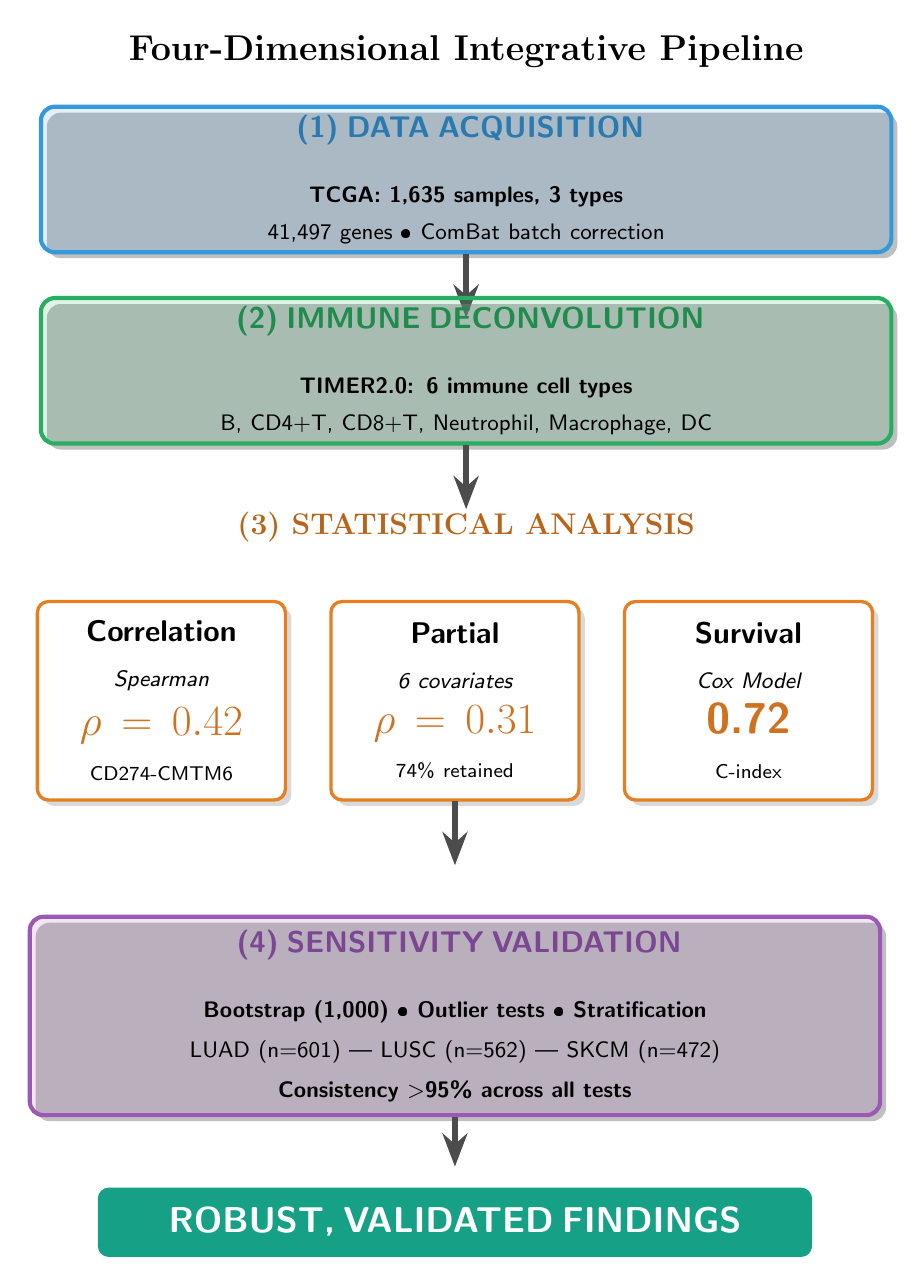
\begin{tikzpicture}[node distance=1.5cm, font=\sffamily, scale=0.9, transform shape]

% Title
\node[font=\Large\bfseries] (title) at (0, 10) {Four-Dimensional Integrative Pipeline};

% Module 1: Data Acquisition - UNIFIED FORMAT
\node[modulebox, fill=datacolor, draw=datacolor] (module1) at (0, 8.2) {
    \vspace{6pt}
    {\large\bfseries\color{datacolor!80!black} (1) DATA ACQUISITION}\\[8pt]
    {\small\textbf{TCGA: 1,635 samples, 3 types}}\\[3pt]
    {\small 41,497 genes • ComBat batch correction}
};

% Arrow 1
\draw[arrow] (module1.south) -- ++(0, -0.9);

% Module 2: Immune Deconvolution - UNIFIED FORMAT
\node[modulebox, fill=immunecolor, draw=immunecolor] (module2) at (0, 5.5) {
    \vspace{6pt}
    {\large\bfseries\color{immunecolor!80!black} (2) IMMUNE DECONVOLUTION}\\[8pt]
    {\small\textbf{TIMER2.0: 6 immune cell types}}\\[3pt]
    {\small B, CD4+T, CD8+T, Neutrophil, Macrophage, DC}
};

% Arrow 2
\draw[arrow] (module2.south) -- ++(0, -0.9);

% Module 3 Title
\node[font=\large\bfseries, color=analysiscolor!80!black] (module3title) at (0, 3.3) {(3) STATISTICAL ANALYSIS};

% Track A - Correlation
\node[trackbox, draw=analysiscolor, below=0.7cm of module3title, xshift=-4.3cm] (trackA) {
    {\large\bfseries Correlation}\\[6pt]
    {\small\itshape Spearman}\\[6pt]
    {\LARGE\bfseries\color{analysiscolor!90!black} $\rho = 0.42$}\\[6pt]
    {\footnotesize CD274-CMTM6}
};

% Track B - Partial Correlation
\node[trackbox, draw=analysiscolor, right=0.6cm of trackA] (trackB) {
    {\large\bfseries Partial}\\[6pt]
    {\small\itshape 6 covariates}\\[6pt]
    {\LARGE\bfseries\color{analysiscolor!90!black} $\rho = 0.31$}\\[6pt]
    {\footnotesize 74\% retained}
};

% Track C - Survival
\node[trackbox, draw=analysiscolor, right=0.6cm of trackB] (trackC) {
    {\large\bfseries Survival}\\[6pt]
    {\small\itshape Cox Model}\\[6pt]
    {\LARGE\bfseries\color{analysiscolor!90!black} 0.72}\\[6pt]
    {\footnotesize C-index}
};

% Arrow 3
\draw[arrow] (trackB.south) -- ++(0, -0.9);

% Module 4: Sensitivity Analysis - FIXED: Proper text width and line breaks
\node[modulebox, fill=validcolor, draw=validcolor, below=1.6cm of trackB, minimum height=2.8cm, text width=11.5cm] (module4) {
    \vspace{6pt}
    {\large\bfseries\color{validcolor!80!black} (4) SENSITIVITY VALIDATION}\\[8pt]
    {\small\textbf{Bootstrap (1,000) • Outlier tests • Stratification}}\\[4pt]
    {\small LUAD (n=601) — LUSC (n=562) — SKCM (n=472)}\\[4pt]
    {\small\bfseries Consistency $>$95\% across all tests}
};

% Arrow to final result
\draw[arrow] (module4.south) -- ++(0, -0.7);

% Final Result Box - FIXED: White text for better contrast
\node[finalbox, fill=resultcolor, draw=resultcolor, below=1cm of module4] (result) {
    {\Large\bfseries\color{white} ROBUST, VALIDATED FINDINGS}
};

\end{tikzpicture}

\end{document}
